\documentclass[11pt,compress,t,n
otes=noshow, aspectratio=169, xcolor=table]{beamer}
% alternatively combining latex files with subfile package https://tex.stackexchange.com/a/155883/26830 (however, page numbering and some other stuff does not work well)

% deactivate beamer navigation
%\setbeamertemplate{navigation symbols}{}
%\usepackage{geometry}
%\geometry{papersize={180mm, 135mm}, top=-1.5mm} % 210mm, 297mm

% set path of iml lecture here, e.g., relative to the current dir
\newcommand{\pathiml}{../}
\usepackage[nospeakermargin]{\pathiml/style/lmu-lecture-combine}
\usepackage{pax}
\setbeamertemplate{frametitle}{\expandafter\uppercase\expandafter\insertframetitle}
%\useoutertheme{metropolis}
% remove section slides
\AtBeginSection[]
{
	\begin{frame}<beamer>
		\frametitle{Advanced Machine Learning}
		\tableofcontents[currentsection, subsectionstyle=hide]
	\end{frame}
}
% includepdf slides, pagecommad will set counter for framenumber
\usepackage{pdfpages}
% if speakermargin, use this
%\includepdfset{trim=0mm 0mm 0mm 0mm, pagecommand={\global\setcounter{framenumber}{\value{page}}}}
% if nospeakermargin, use this
\includepdfset{trim=0mm 0mm 42.6666666667mm 0mm, pagecommand={\global\setcounter{framenumber}{\value{page}}}}
% trim=0mm 6mm 0mm 0mm, offset=0 15,
% add footer:
\usepackage{framed, color}
\usepackage{xcolor}

\newif\ifchapterslideno
\chapterslidenofalse % default: footline shows only total number
%\chapterslidenotrue % alternative: footline shows total and chapter no

\ifchapterslideno
% ---- Alternative footline ----
\usepackage{calc}
\usepackage{transparent} % (optional, for your transparent page numbers)
\setbeamertemplate{footline}[text line]{%
	\noindent\hspace*{\dimexpr-\oddsidemargin-1in\relax}%
	\colorbox{white}{
		\makebox[\dimexpr\paperwidth-9ex\relax]{
			\color{black}
			\begin{minipage}[c][2.5ex][b]{0.5\linewidth}
				\secname
			\end{minipage}
			\hfill\begin{minipage}[c][2.5ex][b]{0.5\linewidth}
				\flushright
				%\insertframenumber{}~/~\inserttotalframenumber~~
			\end{minipage}
	}}%
	\begin{minipage}[c][3.5ex][t]{6.5ex}
		\flushright
		\fontsize{4pt}{6}\selectfont\transparent{0.3}\insertframenumber{}~/~\inserttotalframenumber~~
	\end{minipage}
	\hspace*{-\paperwidth}
}
\else
% ---- Default footline ----
\setbeamertemplate{footline}[text line]{%
	\noindent\hspace*{\dimexpr-\oddsidemargin-1in\relax}%
	\colorbox{white}{
		\makebox[\dimexpr\paperwidth-2\fboxsep\relax]{
			\color{black}
			\begin{minipage}[c][2.5ex][b]{0.5\linewidth}
				\secname
			\end{minipage}
			\hfill\begin{minipage}[c][2.5ex][b]{0.5\linewidth}
				\flushright
				\insertframenumber{}~/~\inserttotalframenumber~~
			\end{minipage}
	}}%
	\hspace*{-\paperwidth}
}
\fi

% \setbeamertemplate{footline}[text line]{%
	%     \noindent\hspace*{\dimexpr-\oddsidemargin-1in\relax}%
	%      \colorbox{white}{
		%      \makebox[\dimexpr\paperwidth-2\fboxsep\relax]{
			%      \color{black}
			%      \begin{minipage}[c][4.5ex][c]{0.5\linewidth}
				%        \secname
				%      \end{minipage}
			%      \hfill\begin{minipage}[c][4.5ex][c]{0.5\linewidth}
				%        \flushright
				%        \insertframenumber{}~/~\inserttotalframenumber~~
				%      \end{minipage}
			%      }}%
	%   \hspace*{-\paperwidth}
	% }
%\fi

\begin{document}
	\setbeamercolor{background canvas}{bg=}

% General remark: hyperlinks in included pdfs are not clickable anymore in the combined pdf unless you use pax to extract annotations from original files and complile this file locally (see https://tex.stackexchange.com/questions/497624/merging-multiple-pdf-files-without-breaking-hyperlinks)


% \section{Shapley Values - Game Theory}
% 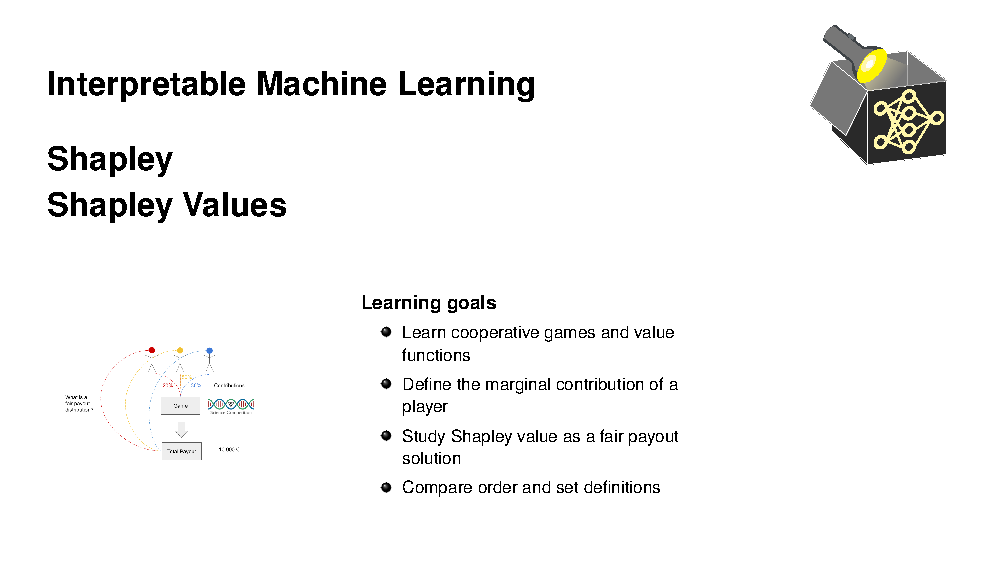
\includepdf[pages={1-last}]{slides01-shapley-game-theory.pdf}
% 
% \section{Shapley Values - Local Feature Effects}
% 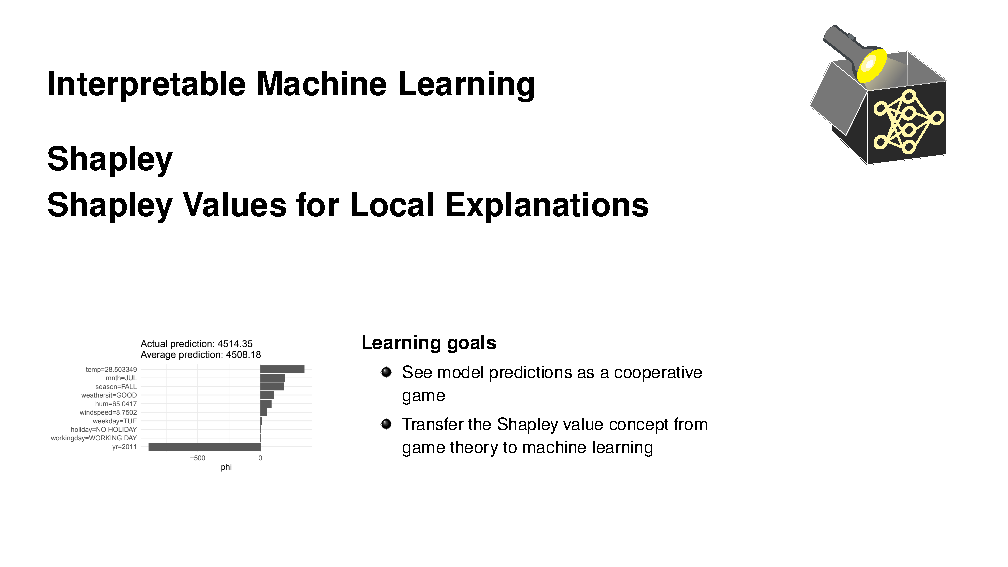
\includepdf[pages={1-last}]{slides02-shapley-ml.pdf}

\section{Intro Feature Importance}
\includepdf[pages={2-8}]{slides01-fi-intro}

\section{Permutation Feature Importance}
\includepdf[pages={2-24}]{slides02-fi-pfi}
\includepdf[pages={3-10}]{slides02-fi-pimp}

\section{Conditional Feature Importance}
\includepdf[pages={3, 5-7, 14}]{slides03-fi-cfi}

\section{Leave One Covariate Out}
\includepdf[pages={2-7, 10, 14}]{slides05-fi-loco}

\end{document}
